

\section{Beispiel 1}

\subsection{Schaltung 1}

Bei der Simulation der Schaltung 1 mittels DC Analyse tritt folgendes Problem auf. In der 
Schleife bestehend aus (L1, C1, R2, R3 und I1) befindet sich eine Gleichstromquelle und ein Kondensator.
Da sich bei einem idelen Kondensator bei diesem Aufbau kein Arbeitspunkt einstellt, sondern die Spannung
bis ins Unendlichen ansteigen würde, ist die Simulation mittels DC-Analyse nicht möglich.

PSPICE gibt dabei folgende Fehlermeldung aus:

\begin{verbatim}
ERROR  PSpiceAD  02:53PM    Node $N_0003 is floating
ERROR  PSpiceAD  02:53PM    Node $N_0005 is floating
\end{verbatim}


\subsection{Schaltung 2}

Eine Simulation der Schaltung 2 funktioniert hingegen Problemlos. Die aus der Simulation hervorgegangenen
Arbeitspunkte können in Abbildung \ref{fig:schalt2_ap} abgelesen werden.


\begin{figure}[h!]
 \centering
 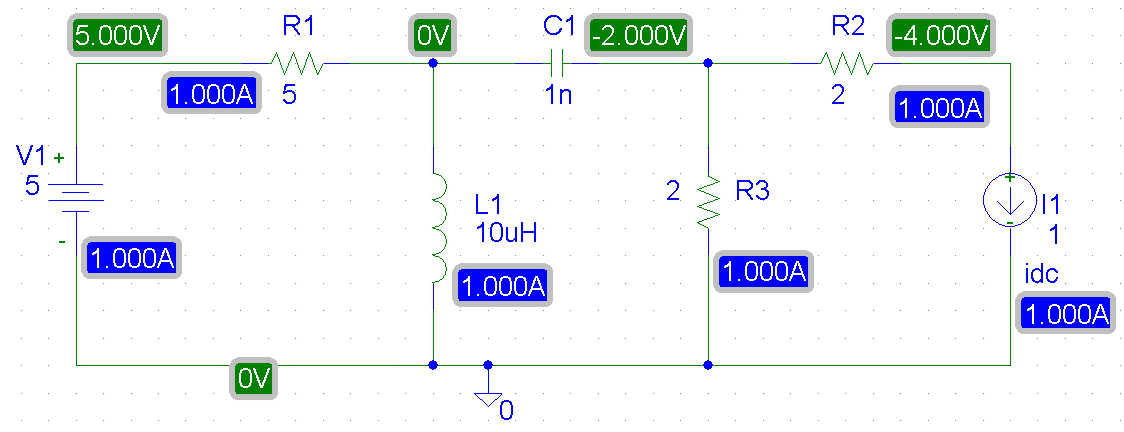
\includegraphics[width=16cm,keepaspectratio=true]{./fig/schalt2_ap.png}
 % schalt2_ap.png: 1124x432 pixel, 72dpi, 39.65x15.24 cm, bb=0 0 1124 432
 \caption{Schaltung 2: Arbeitspunkte aus Simulation}
 \label{fig:schalt2_ap}
\end{figure}


\subsection{Berechnung mittels Knotenpotentialverfahrens}

Bei der Berechnung mittels modifiziertem Knotenpotentialverfahrens (DC) werden zunächst alle
Kapazitäten durch Leerläufe und alle Induktivitäten durch Kurzschlüsse ersetzt.



\begin{figure}[h!]
 \centering
 \includegraphics[width=16cm,keepaspectratio=true]{./fig/schalt2_mpkv.png}
 % schalt2_ap.png: 1124x432 pixel, 72dpi, 39.65x15.24 cm, bb=0 0 1124 432
 \caption{Schaltung 2: modifiziertes Knotenpotentialverfahren, Induktivitäten ersetzt durch Kurzschluss, Kondensatoren ersetzt durch Leerlauf.}
 \label{fig:schalt2_mpkv}
\end{figure}
